\documentclass[]{article}
\usepackage[a4paper, total={15cm,23cm}]{geometry}
\usepackage{fancyhdr}
\usepackage{graphicx}
\usepackage{amsmath}
\usepackage{amssymb}
\usepackage{xcolor}
\usepackage{tikz}
\usepackage{verbatim}
\usepackage{tcolorbox}
\usepackage{textcomp}
\usepackage{xcomment}
\usepackage{xstring}
\usepackage{array}
%opening
\title{PH 221 Week 1}
\author{Benjamin Bauml}
\date{Winter 2025}
\pagestyle{fancy}
\rhead{PH 221}
\chead{Winter 2025}
\lhead{Week 1}

% Version 2024-02-21
% Changes
% 2024-02-21 Added xstring package to enable smooth implementation of new \ModePage command.
% For Assignment, leave Purpose as 1. For Worksheet, set to 2. For Student Solution, set to 3. For Teacher Solution, set to 4.
\newcommand{\Purpose}{1}

\newcommand{\Exclusion}{0}
\newcommand{\PageTurn}{0}
\newcommand{\GrayProb}{0}
\newcommand{\Tipsy}{0}

% Assignment
\if\Purpose1
\renewcommand{\Exclusion}{1}
\fi
% Worksheet
\if\Purpose2
\renewcommand{\Exclusion}{1}
\renewcommand{\PageTurn}{1}
\fi
% Student Solution
\if\Purpose3
\renewcommand{\PageTurn}{1}
\renewcommand{\GrayProb}{1}
\fi
% Teaching Copy
\if\Purpose4
\renewcommand{\PageTurn}{1}
\renewcommand{\GrayProb}{1}
\renewcommand{\Tipsy}{1}
\fi

\if\Exclusion1
\xcomment{Title,Problem,ProblemSub,PassFig}
\fi

\def \NewQ {0}
\def \PForce {0}
\newcommand{\MaybePage}[1]{
	\def \PForce {#1}
	\if\PForce1
		\newpage
	\else
		\if\NewQ0
		\gdef \NewQ {\PageTurn}
		\else
		\newpage
		\fi
	\fi
}

\newcommand{\ModePage}[1]{
	\IfSubStr{#1}{\Purpose}{\newpage}{}
}

\newenvironment{Problem}[2][0]{%The first argument is optional, and if it is set to 1, the \newpage will be forced.
\MaybePage{#1}
\section*{#2}
\if\GrayProb1
\begin{tcolorbox}[colback=lightgray,colframe=lightgray,sharp corners,boxsep=1pt,left=0pt,right=0pt,top=0pt,bottom=0pt,after skip=2pt]
\else
\begin{tcolorbox}[colback=white,colframe=white,sharp corners,boxsep=1pt,left=0pt,right=0pt,top=0pt,bottom=0pt,after skip=2pt]
\fi
}{
\end{tcolorbox}\noindent
}

\newenvironment{ProblemSub}[1][0]{%The argument is optional, and if a string of numbers is entered into it, it will force a \newpage in any \Purpose that shows up in the string. For example, "13" would lead to the newpage being forced in modes 1 and 3.
\ModePage{#1}
\if\GrayProb1
\begin{tcolorbox}[colback=lightgray,colframe=lightgray,sharp corners,boxsep=1pt,left=0pt,right=0pt,top=0pt,bottom=0pt,after skip=2pt]
\else
\begin{tcolorbox}[colback=white,colframe=white,sharp corners,boxsep=1pt,left=0pt,right=0pt,top=0pt,bottom=0pt,after skip=2pt]
\fi
}{
\end{tcolorbox}\noindent
}

\newenvironment{PassFig}{\begin{figure}[h]}{\end{figure}}

\newcommand{\TeachingTips}[1]{
\if\Tipsy1
\begin{tcolorbox}[colback=lightgray,colframe=black]
#1
\end{tcolorbox}
\fi
}

\newenvironment{Title}{\maketitle}{}

\begin{document}
\begin{Title}
\begin{center}
	This material is borrowed/adapted from PH 201 Tutorial 1 for Fall 2020 and the \textit{Learning Introductory Physics with Activities} textbook.
\end{center}
\end{Title}

\begin{Problem}{Activity 1}
	Add or subtract the following vectors.
\end{Problem}
In the solutions below, the first vector is colored {\color{blue}blue}, the second vector {\color{red}red}, and the resultant vector {\color{purple}purple}. Where applicable, both the ``tail-to-tip'' and the ``parallelogram'' method were used.

\begin{PassFig}
	\centering
	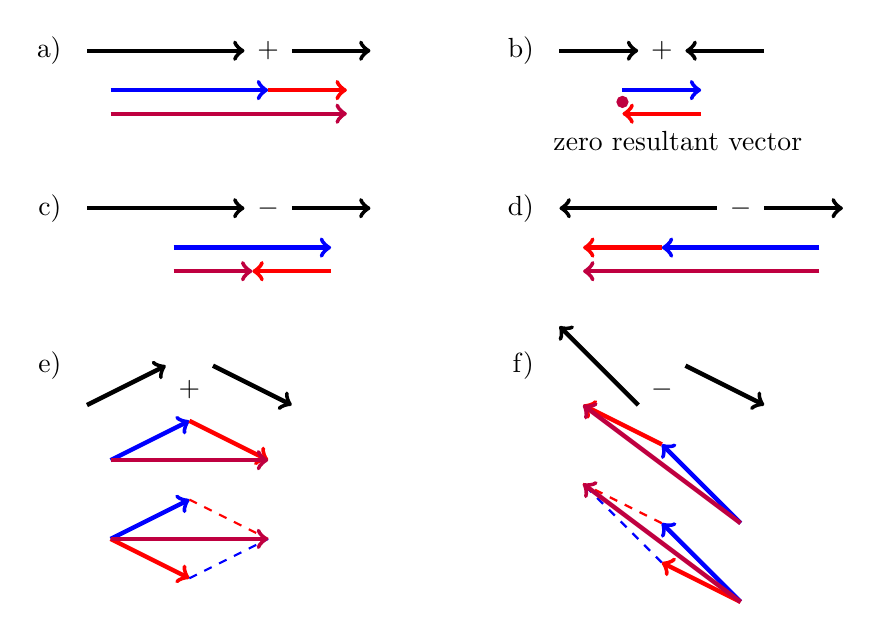
\begin{tikzpicture}
		\begin{scope}[shift={(0,0)}]
			\node[anchor=east] at (0,0) {a)};
			\draw[->,ultra thick,shift={(0.2,0)}] (0,0) -- (2,0);
			\node at (2.5,0) {$+$};
			\draw[->,ultra thick,shift={(2.8,0)}] (0,0) -- (1,0);
			\if\GrayProb1
			\draw[->,blue,ultra thick,shift={(0.5,-0.5)}] (0,0) -- (2,0);
			\draw[->,red,ultra thick,shift={(2.5,-0.5)}] (0,0) -- (1,0);
			\draw[->,purple,ultra thick,shift={(0.5,-0.8)}] (0,0) -- (3,0);
			\fi
		\end{scope}
		\begin{scope}[shift={(6,0)}]
			\node[anchor=east] at (0,0) {b)};
			\draw[->,ultra thick,shift={(0.2,0)}] (0,0) -- (1,0);
			\node at (1.5,0) {$+$};
			\draw[->,ultra thick,shift={(1.8,0)}] (1,0) -- (0,0);
			\if\GrayProb1
			\draw[->,blue,ultra thick,shift={(1,-0.5)}] (0,0) -- (1,0);
			\draw[->,red,ultra thick,shift={(1,-0.8)}] (1,0) -- (0,0);
			\filldraw[purple] (1,-0.65) circle (2pt);
			\node[anchor=north west] at (0,-0.9) {zero resultant vector};
			\fi
		\end{scope}
		\begin{scope}[shift={(0,-2)}]
			\node[anchor=east] at (0,0) {c)};
			\draw[->,ultra thick,shift={(0.2,0)}] (0,0) -- (2,0);
			\node at (2.5,0) {$-$};
			\draw[->,ultra thick,shift={(2.8,0)}] (0,0) -- (1,0);
			\if\GrayProb1
			\draw[->,blue,ultra thick,shift={(1.3,-0.5)}] (0,0) -- (2,0);
			\draw[->,red,ultra thick,shift={(2.3,-0.8)}] (1,0) -- (0,0);
			\draw[->,purple,ultra thick,shift={(1.3,-0.8)}] (0,0) -- (1,0);
			\fi
		\end{scope}
		\begin{scope}[shift={(6,-2)}]
			\node[anchor=east] at (0,0) {d)};
			\draw[->,ultra thick,shift={(0.2,0)}] (2,0) -- (0,0);
			\node at (2.5,0) {$-$};
			\draw[->,ultra thick,shift={(2.8,0)}] (0,0) -- (1,0);
			\if\GrayProb1
			\draw[->,blue,ultra thick,shift={(3.5,-0.5)}] (0,0) -- (-2,0);
			\draw[->,red,ultra thick,shift={(0.5,-0.5)}] (1,0) -- (0,0);
			\draw[->,purple,ultra thick,shift={(0.5,-0.8)}] (3,0) -- (0,0);
			\fi
		\end{scope}
		\begin{scope}[shift={(0,-4)}]
			\node[anchor=east] at (0,0) {e)};
			\draw[->,ultra thick,shift={(0.2,0)}] (0,-0.5) -- (1,0);
			\node at (1.5,-0.3) {$+$};
			\draw[->,ultra thick,shift={(1.8,0)}] (0,0) -- (1,-0.5);
			\if\GrayProb1
			\draw[->,blue,ultra thick,shift={(0.5,-0.7)}] (0,-0.5) -- (1,0);
			\draw[->,red,ultra thick,shift={(1.5,-0.7)}] (0,0) -- (1,-0.5);
			\draw[->,purple,ultra thick,shift={(0.5,-1.2)}] (0,0) -- (2,0);
			\draw[->,blue,ultra thick,shift={(0.5,-1.7)}] (0,-0.5) -- (1,0);
			\draw[->,red,ultra thick,shift={(0.5,-2.2)}] (0,0) -- (1,-0.5);
			\draw[dashed,red,thick,shift={(1.5,-1.7)}] (0,0) -- (1,-0.5);
			\draw[dashed,blue,thick,shift={(1.5,-2.2)}] (0,-0.5) -- (1,0);
			\draw[->,purple,ultra thick,shift={(0.5,-2.2)}] (0,0) -- (2,0);
			\fi
		\end{scope}
		\begin{scope}[shift={(6,-4)}]
			\node[anchor=east] at (0,0) {f)};
			\draw[->,ultra thick,shift={(0.2,0)}] (1,-0.5) -- (0,0.5);
			\node at (1.5,-0.3) {$-$};
			\draw[->,ultra thick,shift={(1.8,0)}] (0,0) -- (1,-0.5);
			\if\GrayProb1
			\draw[->,blue,ultra thick,shift={(1.5,-1.5)}] (1,-0.5) -- (0,0.5);
			\draw[->,red,ultra thick,shift={(1.5,-1)}] (0,0) -- (-1,0.5);
			\draw[->,purple,ultra thick,shift={(2.5,-2)}] (0,0) -- (-2,1.5);
			\draw[->,blue,ultra thick,shift={(1.5,-2.5)}] (1,-0.5) -- (0,0.5);
			\draw[dashed,blue,thick,shift={(0.5,-2)}] (1,-0.5) -- (0,0.5);
			\draw[dashed,red,thick,shift={(1.5,-2)}] (0,0) -- (-1,0.5);
			\draw[->,red,ultra thick,shift={(2.5,-3)}] (0,0) -- (-1,0.5);
			\draw[->,purple,ultra thick,shift={(2.5,-3)}] (0,0) -- (-2,1.5);
			\fi
		\end{scope}
	\end{tikzpicture}
\end{PassFig}

\begin{Problem}{Activity 2}
	In the following figure, the magnitudes of the vectors are $|\vec{a}| = 5$ and $|\vec{b}|=5$. Assume that $\vec{c}=\vec{a}+\vec{b}$ and $\vec{d}=\vec{a}-\vec{b}$.
\end{Problem}
\begin{PassFig}
	\centering
	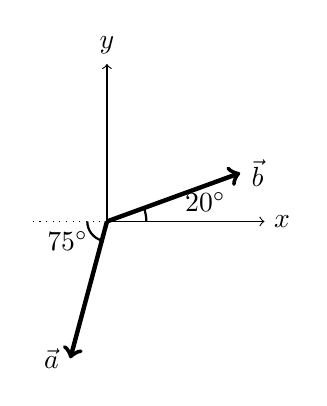
\begin{tikzpicture}
		\draw[<->] (0,2) node[anchor=south] {$y$} -- (0,0) -- (2,0) node[anchor=west] {$x$};
		\draw[->,ultra thick,rotate=20] (0,0) -- (1.8,0) node[anchor=west] {$\vec{b}$};
		\draw[->,ultra thick,rotate=255] (0,0) -- (1.8,0) node[anchor=east] {$\vec{a}$};
		\draw[dotted] (0,0) -- (-1,0);
		\draw[thick] (-0.25,0) arc (180:255:0.25);
		\node[anchor=north] at (-0.5,0) {$75^{\circ}$};
		\draw[thick] (0.5,0) arc (0:20:0.5);
		\node[anchor=south] at (1.25,0) {$20^{\circ}$};
	\end{tikzpicture}
\end{PassFig}
\begin{ProblemSub}
	Determine the magnitude of the vectors $\vec{c}$ and $\vec{d}$. What is the angle to each vector from the positive $x$-axis?
\end{ProblemSub}
To begin, let us make some visual representations of vector addition. We can estimate the quantities in question and use them to validate our final answers.
\begin{figure}[h]
	\centering
	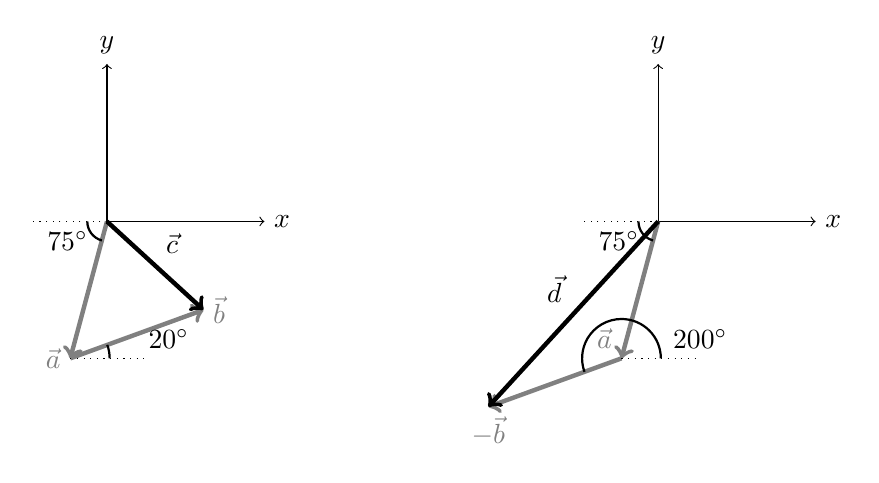
\begin{tikzpicture}
		\begin{scope}
		\draw[<->] (0,2) node[anchor=south] {$y$} -- (0,0) -- (2,0) node[anchor=west] {$x$};
		\draw[->,ultra thick,rotate=255,gray] (0,0) -- (1.8,0) node (atip) {};
		\node[anchor=east,gray] at (atip) {$\vec{a}$};
		\begin{scope}[shift={(atip)}]
		\draw[->,ultra thick,rotate=20,gray] (0,0) -- (1.8,0) node (btip) {};
		\node[anchor=west,gray] at (btip) {$\vec{b}$};
		\draw[thick] (0.5,0) arc (0:20:0.5);
		\node[anchor=south] at (1.25,0) {$20^{\circ}$};
		\draw[dotted] (0,0) -- (1,0);
		\end{scope}
		\draw[dotted] (0,0) -- (-1,0);
		\draw[thick] (-0.25,0) arc (180:255:0.25);
		\node[anchor=north] at (-0.5,0) {$75^{\circ}$};
		\draw[->,ultra thick,rotate=-42.5] (0,0) -- (0.82,0) node[anchor=south west] {$\vec{c}$} -- (1.66,0);
		\end{scope}
		\begin{scope}[shift={(7,0)}]
			\draw[<->] (0,2) node[anchor=south] {$y$} -- (0,0) -- (2,0) node[anchor=west] {$x$};
			\draw[->,ultra thick,rotate=255,gray] (0,0) -- (1.8,0) node (atip) {};
			\node[anchor=south east,gray] at (atip) {$\vec{a}$};
			\begin{scope}[shift={(atip)}]
				\draw[->,ultra thick,rotate=200,gray] (0,0) -- (1.8,0) node (btip) {};
				\node[anchor=north,gray] at (btip) {$-\vec{b}$};
				\draw[thick] (0.5,0) arc (0:200:0.5);
				\node[anchor=south] at (1,0) {$200^{\circ}$};\draw[dotted] (0,0) -- (1,0);
			\end{scope}
			\draw[dotted] (0,0) -- (-1,0);
			\draw[thick] (-0.25,0) arc (180:255:0.25);
			\node[anchor=north] at (-0.5,0) {$75^{\circ}$};
			\draw[->,ultra thick,rotate=227.5] (0,0) -- (1.6,0) node[anchor=south east] {$\vec{d}$} -- (3.19,0);
		\end{scope}
	\end{tikzpicture}
\end{figure}

We can see that $\vec{c}$ will be slightly smaller than 5 units long, and nearly 45$^{\circ}$ below the positive $x$-axis, while $\vec{d}$ will be probably close to 9 units long (almost twice 5, based on my visual estimate) and around 135$^{\circ}$ below the positive $x$-axis.

To begin, let us break down the known vectors into their components. Note that the angle $\vec{a}$ makes is with respect to the negative $x$-axis and below it, so an explicit negative sign will be added both components.
\[
\begin{split}
	a_{x} & = -5\cos(75^{\circ}) \approx -1.29, \\
	a_{y} & = -5\sin(75^{\circ}) \approx -4.83, \\
	b_{x} & = 5\cos(20^{\circ}) \approx 4.70, \\
	b_{y} & = 5\sin(20^{\circ}) \approx 1.71.
\end{split}
\]
Adding the vectors componentwise, we obtain
\[
\begin{split}
	\vec{c} & = \vec{a}+\vec{b} \approx 3.41 \hat{x} - 3.12 \hat{y}, \\
	\vec{d} & = \vec{a}-\vec{b} \approx -5.99 \hat{x} - 6.54 \hat{y}.
\end{split}
\]
We can then use the Pythagorean theorem to calculate the magnitudes of these vectors:
\[
\begin{split}
	|\vec{c}| & \approx \sqrt{3.41^{2}+3.12^{2}} \approx 4.62, \\
	|\vec{d}| & \approx \sqrt{5.99^{2}+6.54^{2}} \approx 8.87.
\end{split}
\]
Trigonometry can be used to find the directions of these vectors. For $\vec{c}$, let the angle from the positive $x$-axis be
\[
\gamma \approx \arctan\left(\frac{-3.12}{3.14}\right) \approx -42.5^{\circ},
\]
therefore $\vec{c}$ points 42.5$^{\circ}$ below the positive $x$-axis. For $\vec{d}$, let the angle from the positive $x$-axis be
\[
\delta^{*} = \approx \arctan\left(\frac{-6.54}{-5.99}\right) \approx 47.5^{\circ}.
\]
However, this points into the first quadrant, which we know is incorrect. The tangent function is tricky that way. It has a period of 180$^{\circ}$, so there is more than one angle that gives the same result, and the inverse tangent is not guaranteed to give you the right one. We can subtract the period to get another valid answer:
\[
\delta = \delta^{*} - 180^{\circ} \approx -132.5^{\circ},
\]
therefore $\vec{d}$ points 132.5$^{\circ}$ below the positive $x$-axis.

\begin{Problem}{Activity 3}
	A semi-truck travels 11 km in 7.5 minutes.
\end{Problem}
\begin{ProblemSub}
	a) What does the ratio (11 km)/(7.5 min) tell you about the truck's motion?
\end{ProblemSub}
This tells us the truck's average speed.
\begin{ProblemSub}
	b) What does the ratio (7.5 min)/(11 km) tell you about the truck's motion?
\end{ProblemSub}
This tells us how long it takes the truck to travel one kilometer.
\begin{ProblemSub}
	c) Find the truck's average speed in miles per hour, then in meters per second. Can you tell what type of road (school zone, residential area, freeway, German Autobahn, etc.) the truck should be traveling on?
\end{ProblemSub}
\[
\begin{split}
	\text{average speed (mph)} & = \frac{11\text{ km}}{7.5\text{ min}} = \frac{11\text{ km}}{7.5\text{ min}} \left(\frac{60 \text{ min}}{1\text{ h}}\right) = 88\text{ km/h} = 88\text{ km/h} \left(\frac{1\text{ mile}}{1.6 \text{ km}}\right) = 55\text{ mph} \\
	\text{average speed (m/s)} & = \frac{11\text{ km}}{7.5\text{ m}} = \frac{11\text{ km}}{7.5\text{ m}} \left(\frac{1000\text{ m}}{1\text{ km}}\right) \left(\frac{1\text{ min}}{60\text{ s}}\right) = 24.444 \text{ m/s} \approx 24\text{ m/s}
\end{split}
\]
55 mph is an appropriate freeway speed for a semi-truck.

Side Note: Notice that I truncated 24.444 to just 24. When figuring out how many decimal places to use, a decent rule of thumb (at this level) is to only include as many digits (not including leading zeros) as you are given in the least precise piece of data. Here, both 11 and 7.5 have two ``significant figures,'' so my final answer should only have two digits. If we had instead been given 11.0 and 7.50, we could assume enough reliability out to three digits to give our final answer as 24.4. However, if we had been given 11.0 and 7.5, we would still want to stick with two digits only, because 7.5 is less precise. Since every data point is assumed to be somewhat uncertain (limited by the accuracy of our measurements), we can't assume that 7.5 is precisely 7.50, nor that 7.50 is precisely 7.500.
\begin{ProblemSub}
	d) Find the time in seconds it takes the truck to travel one meter.
\end{ProblemSub}
\[
\text{time per meter} = \frac{7.5\text{ min}}{11\text{ km}} = \frac{7.5\text{ min}}{11\text{ km}} \left(\frac{1\text{ km}}{1000\text{ m}}\right) \left(\frac{60\text{ s}}{1\text{ min}}\right) = \frac{1}{24.444\text{ m/s}} \approx 0.041\text{ s/m}
\]
Side Note: 0.041 has two ``significant figures,'' since we do not count the leading zeros.


\begin{Problem}{Activity 4}
	Maria hikes 15.0 km at an angle of 30.0$ ^{\circ} $ north of east and then hikes 15.0 km southeast (an angle of 45.0$ ^{\circ} $ south of east). Let Maria's starting point be the origin of your coordinate system, the east-west axis be horizontal, and the north-south axis be vertical with east and north the positive directions.
\end{Problem}
\begin{ProblemSub}
	a) Draw a sketch, approximately to scale, showing the coordinate axes, Maria's two displacements, and her total displacement.
\end{ProblemSub}
\begin{figure}[h]
	\centering
	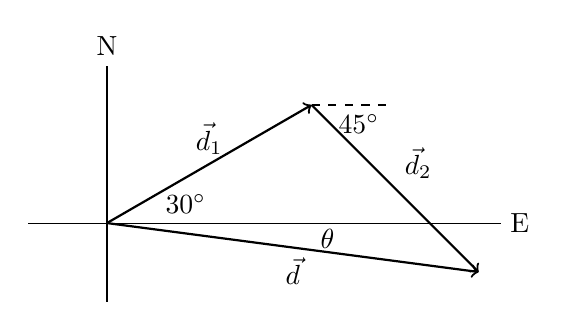
\begin{tikzpicture}
		\draw (0,-1) -- (0,2);
		\node[anchor=south] at (0,2) {N};
		\draw (-1,0) -- (5,0);
		\node[anchor=west] at (5,0) {E};
		\draw[->,thick] (0,0) -- ({3*cos(30)},{3*sin(30)});
		\node[anchor=south] at ({1.5*cos(30)},{1.5*sin(30)}) {$\vec{d}_{1}$};
		\node[anchor=south] at (1,0) {$30^{\circ}$};
		\draw[dashed] ({3*cos(30)},{3*sin(30)}) -- ({3*cos(30)+1},{3*sin(30)});
		\node[anchor=north] at ({3*cos(30)+0.6},{3*sin(30)}) {$45^{\circ}$};
		\draw[->,thick] ({3*cos(30)},{3*sin(30)}) -- ({3*cos(30)+3*cos(45)},{3*sin(30)-3*sin(45)});
		\node[anchor=south west] at ({3*cos(30)+1.5*cos(45)},{3*sin(30)-1.5*sin(45)}) {$\vec{d}_{2}$};
		\draw[->,thick] (0,0) -- ({3*cos(30)+3*cos(45)},{3*sin(30)-3*sin(45)});
		\node[anchor=north] at ({1.5*cos(30)+1.5*cos(45)},{1.5*sin(30)-1.5*sin(45)}) {$\vec{d}$};
		\node[anchor=north] at (2.8,0.05) {$\theta$};
	\end{tikzpicture}
\end{figure}

\noindent\textbf{Known:}
\begin{itemize}
	\item $ d_{1} = 15.0\text{ km};\ \theta_{1} = 30.0^{\circ} $
	\item $ d_{2} = 15.0\text{ km};\ \theta_{2} = -45.0^{\circ} $
\end{itemize}
\textbf{Find:} $ d,\ \theta $
\begin{ProblemSub}
	b) Find the east ($ x $) and north ($ y $) components of Maria's two displacements.
\end{ProblemSub}
\[
\begin{split}
	d_{1E} & = d_{1}\cos\theta_{1} = (15.0\text{ km})\cos30.0^{\circ} = 12.99\text{ km} \\
	d_{1N} & = d_{1}\sin\theta_{1} = (15.0\text{ km})\sin30.0^{\circ} = 7.50\text{ km} \\
	d_{2E} & = d_{2}\cos\theta_{2} = (15.0\text{ km})\cos(-45.0^{\circ}) = 10.61\text{ km} \\
	d_{2N} & = d_{2}\sin\theta_{2} = (15.0\text{ km})\sin(-45.0^{\circ}) = -10.61\text{ km} \\
\end{split}
\]
\begin{ProblemSub}
	c) Find the east ($ x $) and north ($ y $) components of Maria's total displacement.
\end{ProblemSub}
\[
\begin{split}
	d_{E} & = d_{1E} + d_{2E} = 12.99\text{ km} + 10.61\text{ km} = 23.60\text{ km} \\
	d_{N} & = d_{1N} + d_{2N} = 7.50\text{ km} + (-10.61\text{ km}) = -3.11\text{ km} \\
\end{split}
\]
\begin{ProblemSub}
	d) Find the magnitude and direction of Maria's total displacement.
\end{ProblemSub}
\[
\begin{split}
	d & = \sqrt{d_{E}^{2}+d_{N}^{2}} = \sqrt{(23.60\text{ km})^{2} + (-3.11\text{ km})^{2}} = 23.8\text{ km} \\
	\theta & = \tan^{-1}\left(\frac{d_{N}}{d_{E}}\right) = \tan^{-1}\left(\frac{-3.11\text{ km}}{23.60\text{ km}}\right) = -7.50^{\circ}
\end{split}
\]
\begin{ProblemSub}
	e) Check your answer to (d) against your sketch. Do they agree?
\end{ProblemSub}
Maria's displacement was 23.8 km at an angle of 7.50$ ^{\circ} $ south of east. This agrees with the sketch which shows a small angle below the x-axis. Note that the magnitude of her total displacement is only slightly greater than her total horizontal displacement because the angle is small.

In adding vectors by components, it is important to keep track of their signs. If we hadn’t had the negative sign in the north component of Maria’s second hike, our answer would have been much different (and wrong).

\begin{Problem}{Activity 5}
	Three vectors add together to equal 0. One vector has magnitude 3 and points in the positive $x$-direction; a second vector has magnitude 5 and points at 120$^{\circ}$ from the positive $x$-axis. Determine the third vector as a magnitude and direction.
\end{Problem}
Below, I have drawn the two vectors---I'm calling the first vector along the $x$-axis $\vec{a}$, and the angled vector $\vec{b}$. A cyan copy of $\vec{b}$ has been placed at the tip of $\vec{a}$ to illustrate the sum $\vec{a}+\vec{b}$. The red vector is what the third vector needs to be for the three to sum to zero.
\begin{figure}[h]
	\centering
	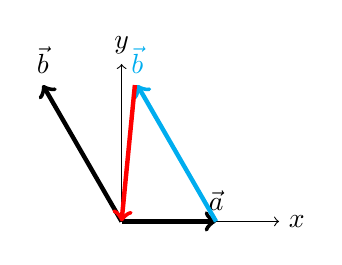
\begin{tikzpicture}
		\draw[<->] (0,2) node[anchor=south] {$y$} -- (0,0) -- (2,0) node[anchor=west] {$x$};
		\draw[->,ultra thick] (0,0) -- (1.2,0) node[anchor=south] {$\vec{a}$};
		\draw[->,ultra thick,rotate=120] (0,0) -- (2,0) node[anchor=south] {$\vec{b}$};
		\draw[->,ultra thick,shift={(1.2,0)},rotate=120,cyan] (0,0) -- (2,0) node[anchor=south] (btip) {$\vec{b}$};
		\draw[->,ultra thick,red] (btip) -- (0,0);
	\end{tikzpicture}
\end{figure}
Based on this representation, we can see that the third vector must be a little shorter than $\vec{b}$, and it will point a little more than 90$^{\circ}$ clockwise from the positive $x$-axis.

Let's break $\vec{b}$ into components:
\[
\begin{split}
	b_{x} & = 5\cos(120^{0}) =-2.5, \\
	b_{y} & = 5\sin(120^{0}) \approx 4.33.
\end{split}
\]
Adding $\vec{a}$ and $\vec{b}$ componentwise gives us
\[
\vec{a}+\vec{b} \approx 3\hat{x} + \left(-2.5\hat{x} + 4.33\hat{y}\right) = 0.5\hat{x} + 4.33\hat{y},
\]
so the third vector (let's call it $\vec{c}$) will be the negative of this:
\[
\vec{c} = -\left(\vec{a}+\vec{b}\right) = -0.5\hat{x} -4.33\hat{y}.
\]
We can get the magnitude via the Pythagorean Theorem:
\[
|\vec{c}| \approx \sqrt{0.5^{2}+4.33^{2}} \approx 4.36.
\]
The angle can be determined trigonometrically, but most calculators will give you the wrong answer first:
\[
\theta^{*} \approx \arctan\left(\frac{-4.33}{-0.5}\right) \approx 83.4.
\]
This would be the angle for $-\vec{c}$. The tangent function has a period of 180$^{\circ}$, so we can subtract this to get another valid angle in the correct quadrant:
\[
\theta = \theta^{*} - 180^{\circ} \approx -96.6^{\circ}.
\]
\end{document}